% ---------------------------------------------------------------------
% ---------------------------------------------------------------------
% ---------------------------------------------------------------------
\part{Results}
\chapter[Sparse \textit{N}-PLS, a method for variable selection in multiway data sets]{Sparse \textit{N}-PLS, a method for variable selection in multiway data sets}



% ---------------------------------------------------------------------
% ---------------------------------------------------------------------
\section{Sparse \textit{N}-PLS, integration of L1 penalization in the \textit{N}-PLS algorithm}
\label{NPLSpenalization}
As commented in the previous chapter, it is proposed to introduce the L1-penalization in the $N$-PLS algorithm. Since there are three modes, the aim is to perform selection not only on the second mode (variables), but also on the third mode. To this aim, a similar approach to that of \cite{le2008sparse} is used. Briefly, to achieve sparse versions of $\textbf{\text{w}}^\text{J}$ and $\textbf{\text{w}}^\text{K}$ for each latent variable, the soft-thresholding penalty function $\beta_j^{lasso}=sgn(\beta_j^{LS})(|\beta_j^{LS}|-\lambda)^+$ is introduced in the $N$-PLS algorithm right after the SVD at the $\textbf{\text{w}}^\text{J}$ and $\textbf{\text{w}}^\text{K}$ determination. The complete algorithm is as follows \autoref{figura40}:


\vspace{20pt}
Center \textbf{\underline{X}} and \textbf{\underline{Y}}, and unfold \textbf{\underline{X}} (and \textbf{\underline{Y}} when necessary) into a two-way matrix.

Let \textbf{u} be some column of \textbf{Y}, and set \textit{f}=1

\begin{enumerate}
    \item $\textbf{\text{w}}^\text{T}=\textbf{\text{u}}^\text{T}\textbf{\text{X}}/\textbf{\text{u}}^\text{T}\textbf{\text{u}}$
    \item Build \textbf{Z} by refolding \textbf{w} according to the modes dimensions
    \item Determine $\textbf{\text{w}}^\text{J}$ and $\textbf{\text{w}}^\text{K}$ by SVD
    \item L1-penalization inclusion
    \begin{enumerate}
        \item Apply soft-thresholding on $\textbf{\text{w}}^\text{J}$: $\beta_j^{lasso}=sgn(\beta_j^{LS})(|\beta_j^{LS}|-\lambda)^+$ 
        \item Apply soft-thresholding on $\textbf{\text{w}}^\text{K}$: $\beta_j^{lasso}=sgn(\beta_j^{LS})(|\beta_j^{LS}|-\lambda)^+$ 
        \item Input the new \textbf{w} as kronecker($\textbf{\text{w}}^\text{K}, \textbf{\text{w}}^\text{J}$)
    \end{enumerate}
    \item $\textbf{\text{t}}=\textbf{\text{Xw}}/\textbf{\text{w}}^\text{T}\textbf{\text{w}}$
    \item $\textbf{\text{q}}=\textbf{\text{Y}}^\text{T}\textbf{\text{t}}/\text{norm}(\textbf{\text{Y}}^\text{T}\textbf{\text{t}})$
    \item $\textbf{u}=\textbf{Yq}$
    \item Check for convergence. If it is achieved, continue; otherwise, go to 1
    \item $\textbf{\text{b}} = (\textbf{\text{T}}^\text{T}\textbf{\text{T}})^{-1}\textbf{\text{T}}^\text{T}\textbf{\text{u}} \text{; where} \ \textbf{\text{T}}=[\text{t1}\ \text{t2} \text{…} \text{t}_f]$
    \item $\textbf{\text{X}} = \textbf{\text{X}}-\textbf{\text{tw}}^\text{T} \ \text{and} \ \textbf{\text{Y}} = \textbf{\text{Y}}-\textbf{\text{tbq}}^\text{T}$
    \item \textit{f} = \textit{f}+1. Continue from step 1 until a good description of \textbf{Y}
\end{enumerate}
\vspace{20pt}

This algorithm is applicable to both the standard regression (continuous response) and the discriminant version of the $N$-PLS model, i.e. $N$-PLS-DA. In the case of $N$-PLS-DA, \textbf{\underline{Y}} is a \textbf{y} vector formed by ones and zeros, each of the two values related to one of the two classes to be segregated. 

\begin{figure}[hbtp]
\centering
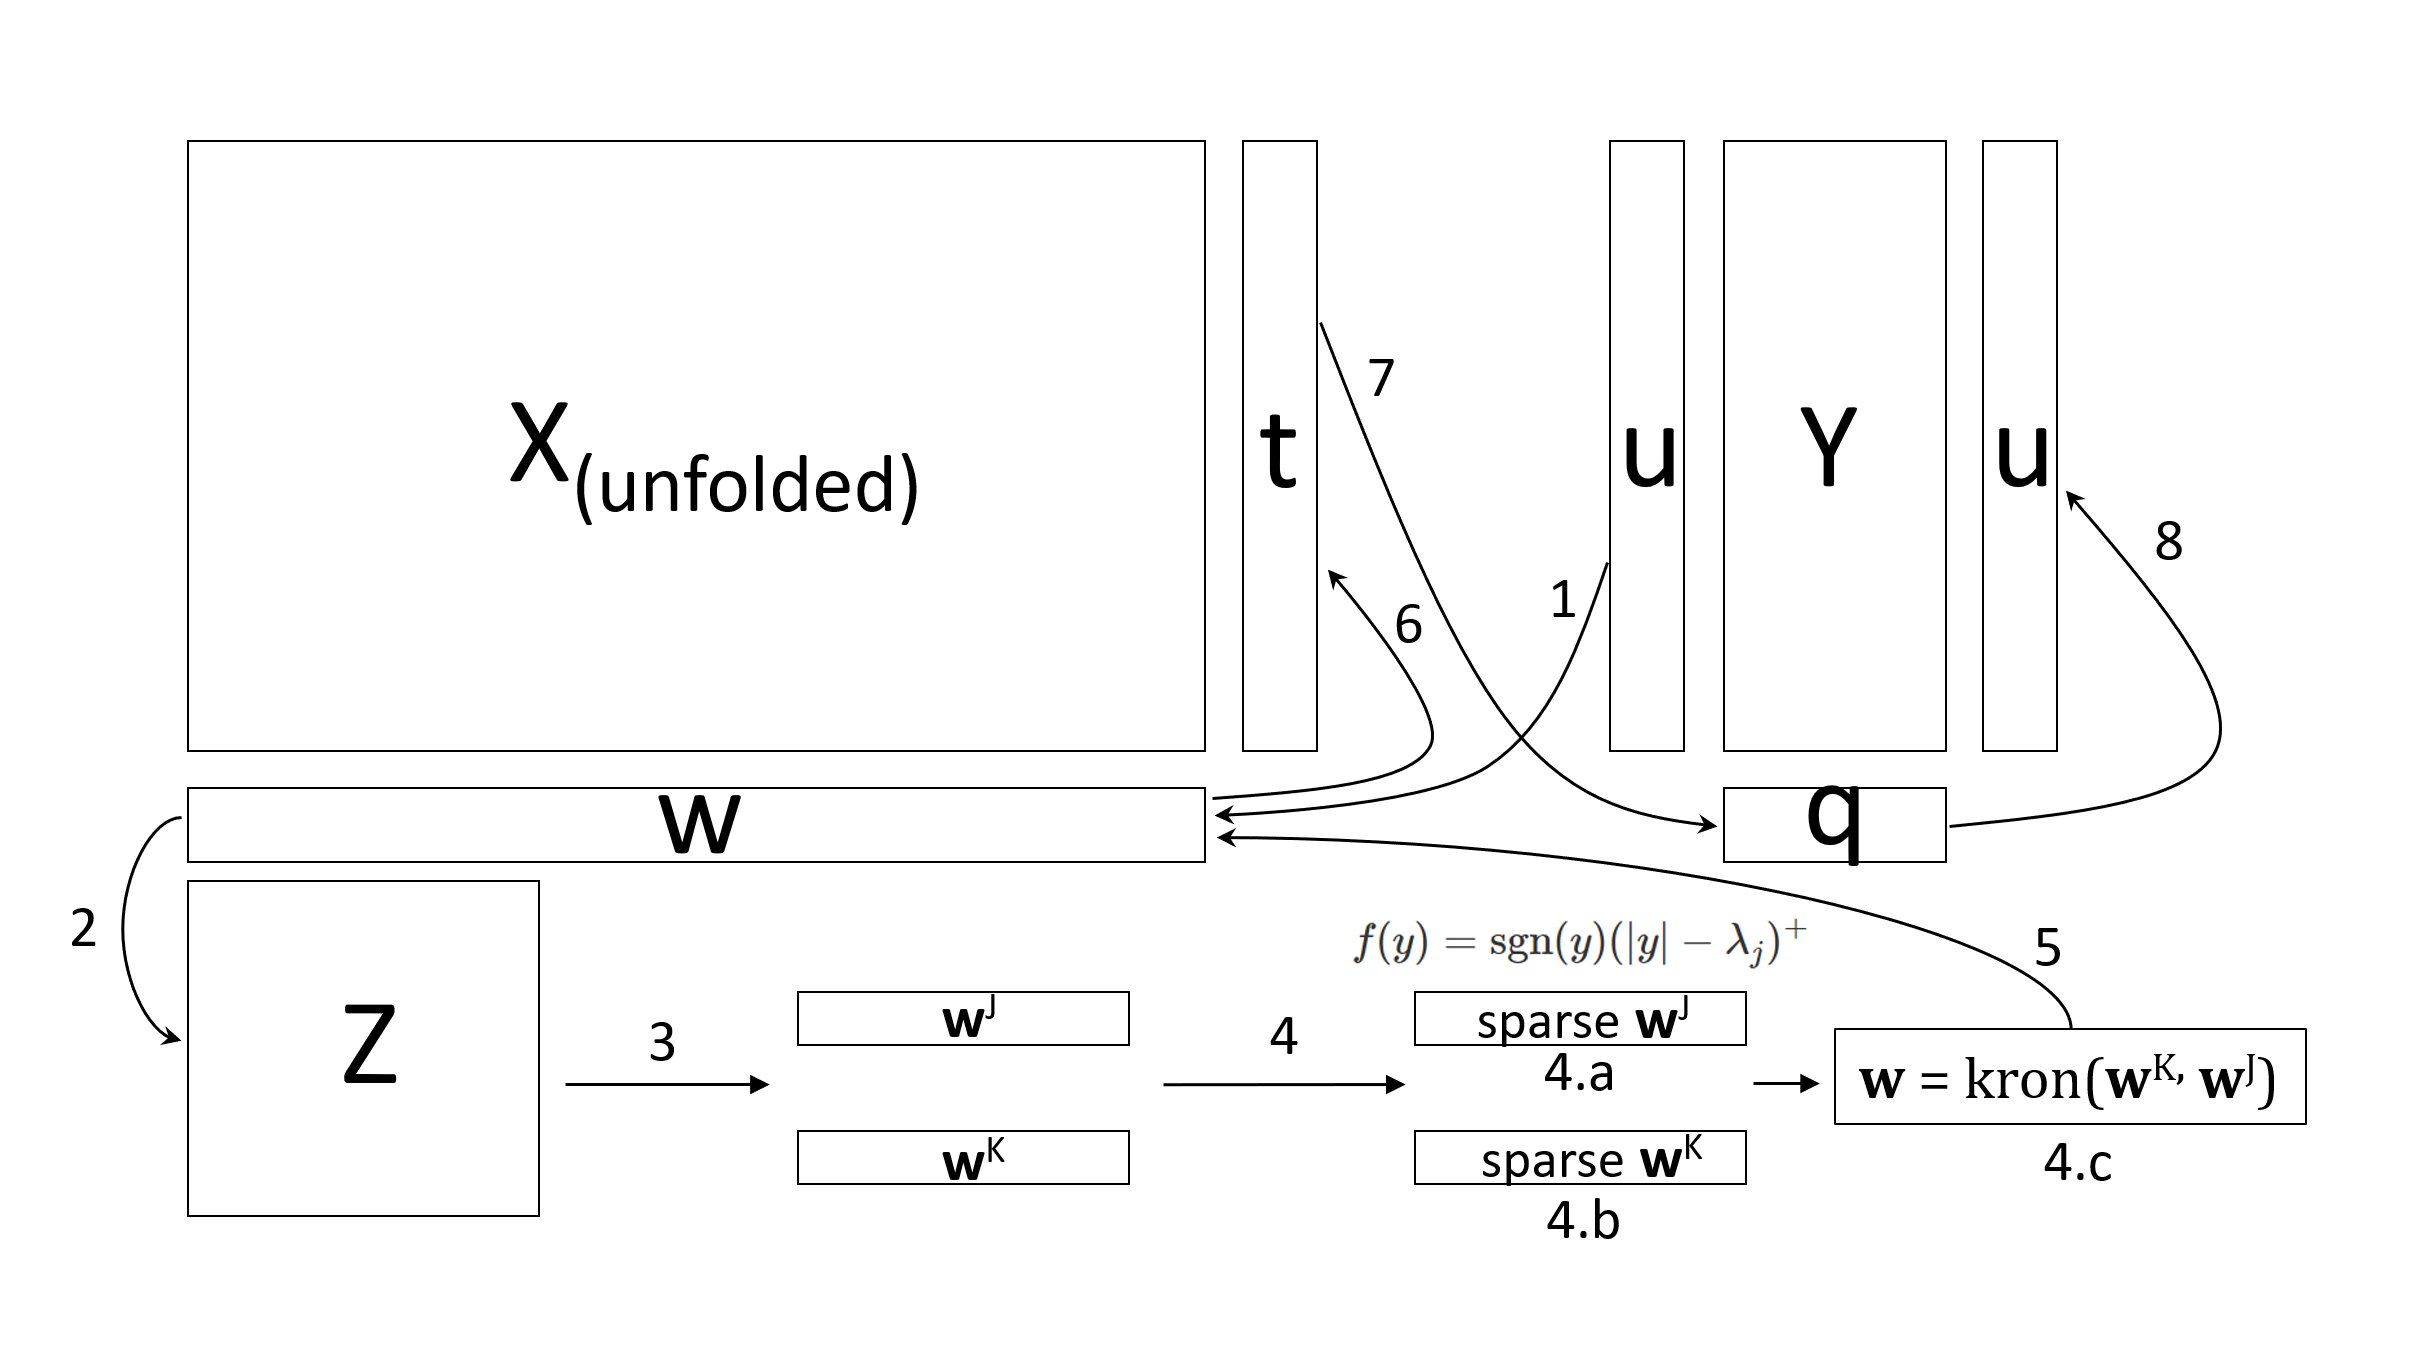
\includegraphics[width=1\textwidth]{figura40.png}
\caption[Scheme detailing the different steps of the sNPLS algorithm]{Scheme detailing the different steps of the sNPLS algorithm as explained in the previous page. \vspace{15pt}}
\label{figura40}
\end{figure}



\section{Hyperparameters of the sparse \textit{N}-PLS algorithm}
\label{hyperparameters}
Hyperparameters are tuneable parameters of the model, whose values are specified before starting the algorithm instead of determined inside the algorithm as standard parameters. L1-penalization has one hyperparameter, called the penalization factor (the amount of L1-penalization to apply). However, since the L1-penalization is applied to both $\textbf{\text{w}}^\text{J}$ and $\textbf{\text{w}}^\text{K}$ the number of hyperparameters for a sparse $N$-PLS model (sNPLS) is three: the number of components (shared with the standard $N$-PLS model), the number of variables to select at each component, and the number of elements of the third mode to select at each component. The number of components can range between one and $J$, and the number of variables per component or elements of the third mode per component can range between zero and $J$ and zero and $K$, respectively. It is necessary that at least one component includes one selected variable and one element of the third mode to fit a valid model. A sparse $N$-PLS model where all variables and all elements of the third mode are forced to be selected reduces to a general $N$-PLS model, where only the number of components acts as hyperparameter.

\subsection{Tuning of the parameters}
Optimization of the hyperparameter values is necessary to achieve optimal prediction power or optimal variable selection performance in the case of sNPLS. One important point to take into account is that consistency (selecting the right variables) and minimizing prediction error appear to be non-compatible \parencite{yang2005can}, so the tuning criterion has to be adapted depending on the main objective of the analysis. For the objective of variable selection, \textcite{zou2005regularization} mention the option of just choosing the desired number of non-zero coefficients as a viable alternative for interpretation purposes. In the present approach, the focus is set on minimizing prediction error, so to perform this tuning of the parameters, a grid search of the hyperparameter space \parencite{lameski2015svm} is proposed guided by the mean squared prediction error evaluated by cross-validation \parencite{duarte2017empirical}. More specifically, the approach consists on performing $K$-fold cross-validation repeatedly and averaging their results, to alleviate instability in the selection of parameters because of high variance in the single cross-validation results \parencite{krstajic2014cross}. This high variance entails that different runs of the cross-validation procedure can yield different results regarding the estimated best set of the parameters and also that the estimation of the best set of parameters is prone to overfitting (bias-variance tradeoff).

Briefly, K-fold cross-validation consists on randomly splitting the data set in a number of folds, $K$, and perform $K$ iterations of model fitting and testing, where a different fold is used as test set in each iteration while the other folds are used to train the model. This way, an out-of-sample estimate for the prediction error of the model is estimated at each iteration. Later, all estimates are averaged to get the mean cross-validated error. 

The procedure is performed as follows:
\vspace{20pt}
\begin{enumerate}
    \item Divide the data set in K subsets (ideally of equal size)
    \item For each k in 1, \dots K:
    \begin{itemize}
        \item Train the model on $(x_i, y_i)$ where $i \notin F_k$
        \item Estimate prediction error on $(x_k, y_k)$ as $E_k$
    \end{itemize}
    \item Average all errors to get the $CVE$ estimate
\end{enumerate}

\vspace{20pt}
A scheme of the procedure for K-fold cross-validation is represented in \autoref{figura39}.

\begin{figure}[hbtp]
\centering
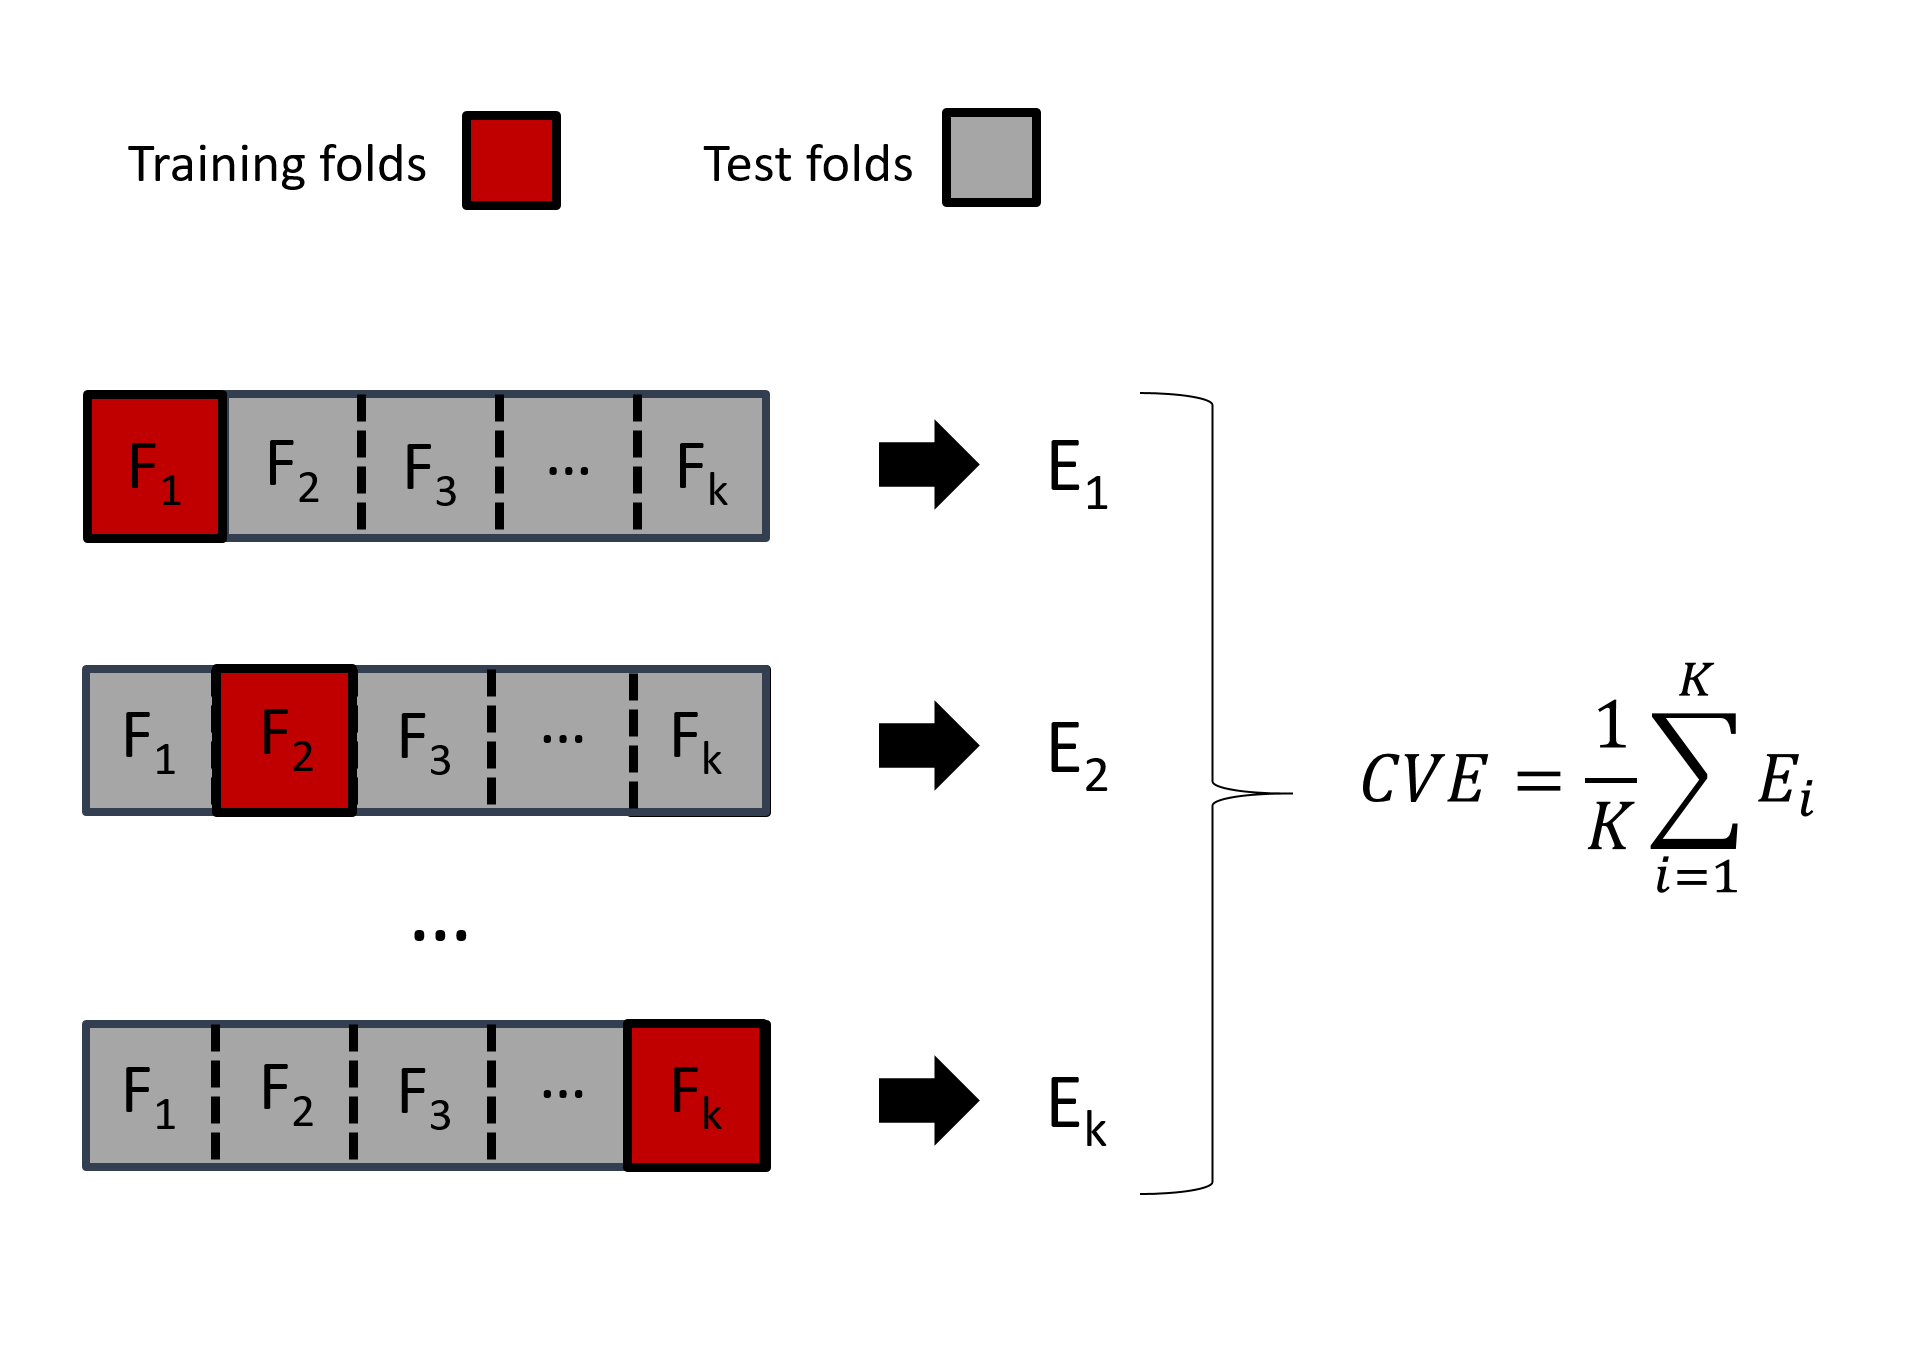
\includegraphics[width=0.7\textwidth]{figura39.png}
\caption[Scheme of a K-fold cross-validation procedure]{Scheme of a K-fold cross-validation procedure. At each iteration, one different fold acts as test fold while all the others act as training folds. At the end, the different prediction errors are averaged.}
\label{figura39}
\end{figure}


There are alternative ways to select or tune the hyperparameters apart from cross-validation \parencite{vujavcic2015computationally, zhang2010regularization}. These alternatives have the advantage of being computationally faster than cross-validation, but one important advantage of cross-validation is the possibility to estimate the standard error of the estimated cross-validated error performing the following steps: 

\vspace{15pt}
\begin{enumerate}
    \item \begin{equation}
    E_k=(y - \hat{y})^2
    \end{equation}
    \item \begin{equation}
    CVE=\frac{1}{K}\sum_{i=1}^{K}E_i
    \end{equation}
    \item \begin{equation}
    SD_{CVE}=\sqrt{var(E_1, E_2, \dots, E_k)}
    \end{equation}
    \item \begin{equation}
    SE_{CVE}=\frac{SD_{CVE}}{\sqrt{K}}
    \end{equation}
\label{secve}
\end{enumerate}

Performing a grid search on a three-dimensional hyperparameter step is computationally very demanding, so the fact that grid search is an embarrassingly parallel task \parencite{mcgibbon2016osprey} is exploited to parallelize the cross-validation procedure and be able to perform the repeated cross-validation in a reasonable time for medium and large data sets. Details on the parallelization algorithm will be presented in next chapter.
